\chapter{KIỂM THỬ PHẦN MỀM}
\begin{flushleft}
	\fontsize{12pt}{7pt}\selectfont
	\textit{Chương này sẽ trình bày về quá trình kiểm thử phần mềm cho eXe. Mục đầu tiên sẽ trình bày về chiến lược kiểm thử cùng các giai đoạn kiểm thử. Mục tiếp theo sẽ nêu ra các thử thách trong quá trình kiểm thử, bao gồm thử thách về mặt công nghệ và sự bùng nổ về số lượng mẫu kiểm tra. Mục thứ ba sẽ đưa ra các hướng giải quyết cho các thử thách này và mục cuối cùng là ví dụ một mẫu kiểm tra đã hiện thực.}
\end{flushleft}

\section{Chiến lược kiểm thử}

Selenium Webdriver là công cụ kiểm thử tự động được lựa chọn để kiểm thử cho eXe. Lý do là cả eXe và SCORM Cloud đều được sử dụng trên trình duyệt. Selenium Webdriver có khả năng tương tác rất tốt với mọi đối tượng trên trình duyệt, vì vậy sẽ rất thích hợp để kiểm thử cho toàn bộ quá trình thực hiện.\\

Để sử dụng một bài giảng điện tử cần một quá trình có hai công việc. Công việc thứ nhất là người soạn thảo sẽ sử dụng eXe để soạn thảo bài giảng, thiết kế nội dung cho các bài học, thiết lập các điều kiện cần thiết cho mỗi bài học,... cuối cùng là đóng gói bài giảng theo chuẩn SCORM 2004 và upload lên SCORM Cloud. Công việc thứ hai là người học thực hiện các bài học có trong bài giảng và hoàn thành tất cả bài học này. Toàn bộ quá trình này đều được tự động hóa bằng Selenium Webdriver.\\

Chiến lược kiểm thử sẽ là quá trình kiểm thử tích hợp (Integration Testing) nhằm mục đích mô phỏng toàn bộ quá trình hoạt động để xây dựng và sử dụng một bài giảng điện tử. Đầu tiên Selenium Webdriver sẽ đóng vai trò người soạn thảo, tự động hóa các công việc như soạn thảo bài giảng, thiết kế nội dung cho các bài học, thiết lập các điều kiện cần thiết cho mỗi bài học,... cuối cùng là đóng gói bài giảng theo chuẩn SCORM 2004 và upload khóa học lên SCORM Cloud. Tiếp theo Selenium Webdriver sẽ đóng vai trò người học, tự động hóa việc tham gia vào bài học và hoàn thành các bài học.\\

Mục đích của chiến lược kiểm thử là đảm bảo cho bài giảng điện tử được tạo ra đúng như thiết lập của người soạn thảo. Đầu tiên người soạn thảo sẽ sử dụng eXe để soạn thảo bài giảng, thiết kế nội dung cho các bài học, thiết lập các điều kiện cần thiết cho mỗi bài học,... cuối cùng là đóng gói bài giảng theo chuẩn SCORM 2004, lúc này bài giảng ngoài nội dung còn có các mã SCORM được sinh ra theo như các thiết lập điều kiện của người soạn thảo. Tiếp theo người soạn thảo sẽ upload bài giảng lên SCORM Cloud, lúc này sẽ kiểm tra cho việc mã SCORM có chạy đúng như đã sinh ra hay không.

\newpage

\begin{center}
	\begin{figure}[htp]
		\begin{center}
			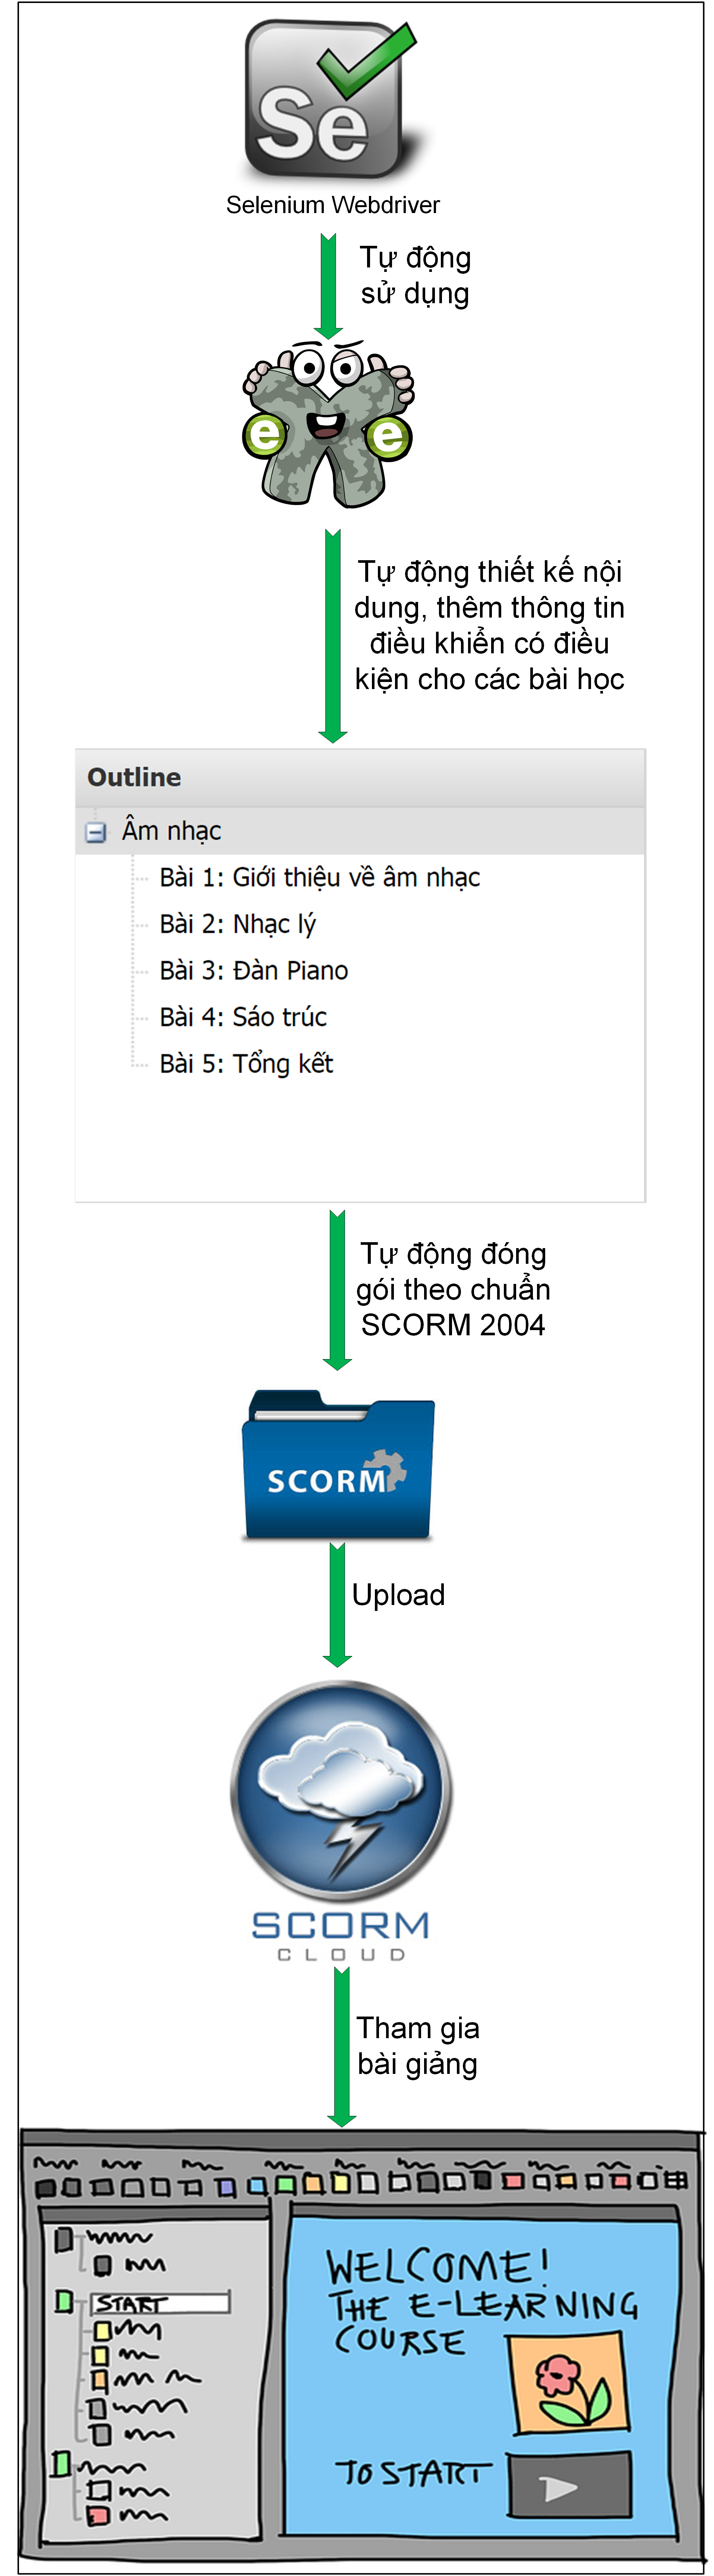
\includegraphics[width=5cm]{Chapter5/Pictures/picture51.png}
		\end{center}
		\caption{Toàn bộ quá trình kiểm thử}
		\label{refhinhchuong71}
	\end{figure}
\end{center}

Hình 5.1 mô tả toàn bộ quá trình kiểm thử tự động. Selenium Webdriver sẽ tự động hóa sử dụng eXe để soạn thảo bài giảng, thiết kế nội dung bài giảng, thiết lập các điều kiện cần thiết cho mỗi bài học, đóng gói bài giảng theo chuẩn SCORM 2004, tiếp theo sẽ upload bài giảng lên SCORM Cloud và tự động tham gia, hoàn thành bài học.
\newpage

\section{Các thử thách trong quá trình kiểm thử}
\subsection{Thử thách về mặt công nghệ}

Thách thức đầu tiên là về mặt thiết kế của eXe. Vì được thiết kế giao diện bằng ExtJS nên eXe sinh ra các đối tượng động. Các đối tượng động ở đây có thể là id, class, button,... hoặc có thể là bất kỳ cặp thẻ HTML nào. eXe còn tự động sinh ra các frame ngẫu nhiên, khiến các đối tượng bị ẩn đi. Những điều này dẫn đến việc xác định các thành phần của eXe rất khó khăn. \\

Thách thức thứ hai là áp dụng kiểm thử tự động cho eXe. Để kiểm thử tự động hiệu quả, chúng ta cần xác định được các thành phần của eXe, tuy nhiên do eXe sinh ra các đối tượng động như trình bày ở trên nên việc này trở nên khó khăn. ExtJS tạo ra những phần tử có cấu trúc phức tạp, có số lượng lớn id hoặc class trùng lặp với nhau. Việc xử lý vấn đề này sẽ được trình bày ở chương sau.\\


\subsection{Thử thách về số lượng mẫu kiểm tra}

Bùng nổ về số lượng mẫu kiểm tra là một vấn đề hết sức phổ biến trong kiểm thử phần mềm. Đa số các phần mềm đều cần có một số lượng mẫu kiểm tra rất lớn để kiểm thử các tính năng của chúng, eXe cũng không phải ngoại lệ và cần phải tìm cách để giảm số lượng mẫu kiểm tra xuống một cách hợp lý.


\begin{comment}
Đối với hướng phát triển thứ nhất, việc kiểm thử bao gồm 2 giai đoạn. Giai đoạn thứ nhất là thiết lập tiền điều kiện (PreCondition) cho mỗi bài học, đây là điều kiện để người học có thể học bài này. Giai đoạn thứ hai là thiết lập hậu điều kiện (PostCondition) cho mỗi bài học, đây là điều kiện để xác định người học hoàn thành bài học này.\\

Giai đoạn thứ nhất là thiết lập tiền điều kiện, chúng ta cần thiết lập thứ tự các bài học để người học tham gia đầy đủ toàn bộ các bài. Sau đây là cách tính các trường hợp có thể xảy ra cho giai đoạn thứ nhất:

\begin{itemize}
\item Một khóa học bao gồm nhiều bài học. Người học cần phải tham gia đầy đủ các bài học thì mới được xem là hoàn thành khóa học.

\item Lấy ví dụ 1 khóa học có 3 bài học, như vậy ta sẽ có 3! = 6 cách thiết lập thứ tự các bài để người học tham gia đầy đủ 3 bài học. Cách thiết lập thứ nhất là người học có thể học bài 1, sau đó đến bài 2 và cuối cùng là bài 3. Cách thiết lập thứ 2 là người học có thể bắt đầu từ bài 2, sau đó học bài 1 và cuối cùng là bài 3,...

\item Một cách tổng quát, đối với 1 khóa học có n bài học thì sẽ có n! cách thiết lập thứ tự các bài để người học hoàn thành khóa học.

\end{itemize}

Như vậy giai đoạn thứ nhất sẽ có số lượng testcase là n!.\\

Giai đoạn thứ hai là thiết lập hậu điều kiện cho mỗi bài học, cần thiết lập điều kiện để xác định người học đã hoàn thành bài học. Có 2 trường hợp được xem là hoàn thành bài học. Trường hợp thứ nhất là người học cần phải ở bài học trong 1 khoảng thời giai nhất định, phải học ở bài học trong khoảng thời giai đã thiết lập thì mới được xem là hoàn thành bài này. Trường hợp thứ hai là phải vượt qua những bài kiểm tra ở bài này, người học cần phải đạt những bài kiểm tra đã quy định thì mới được xem là hoàn thành bài học. Sau đây là cách tính các trường hợp có thể xảy ra cho giai đoạn thứ hai:

\begin{itemize}
\item Trường hợp thứ nhất là phải ở bài học trong khoảng thời giai đã quy định. Đối với trường hợp này chỉ có 2 trường hợp là có thời giai hoặc không có thời giai ở mỗi bài. Như vậy một cách tổng quát, đối với 1 khóa học có n bài học thì sẽ có tổng cộng 2n testcase cho trường hợp này.

\item Trường hợp thứ hai là phải vượt qua những bài kiểm tra đã quy định thì mới được xem là hoàn thành bài học.Có 2 cách thiết lập chính cho trường hợp này. Cách thứ nhất là thiết lập chính xác các bài kiểm tra cần đạt. Cách thứ hai là thiết lập chỉ cần đạt một bài kiểm tra bất kỳ trong các bài kiểm tra này. Sau đây là cách tính cho trường hợp này:
\begin{itemize}
\item Lấy ví dụ một bài học có 3 bài kiểm tra, với cách thứ nhất là cần đạt những bài kiểm tra đã thiết lập, chúng ta có những trường hợp sau đây:

\begin{itemize}
\item Nếu thiết lập cần đạt 1 bài kiểm tra trong 3 bài này thì sẽ có tổ hợp 1 trong 3 bài này, tức $C_3^1$ = 3 cách thiết lập. Cách thiết lập thứ nhất là đạt bài 1, cách thiết lập thứ 2 là đạt bài 2 và cách thiết lập thứ 3 là đạt bài 3. Một cách tổng quát, để thiết lập cần đạt 1 bài kiểm tra trong m bài kiểm tra thì trong trường hợp này sẽ có $C_m^1$ cách thiết lập.

\item Nếu thiết lập cần đạt 2 bài kiểm tra trong 3 bài này thì sẽ có tổ hợp 2 trong 3 bài này, tức $C_3^2$ = 3 cách thiết lập. Cách thiết lập thứ nhất là cần đạt bài 1 và bài 2, cách thiết lập thứ hai là cần đạt bài 2 và bài 3 và cách thiết lập thứ ba là cần đạt bài 1 và bài 3. Một cách tổng quát, để thiết lập cần đạt 2 bài kiểm tra trong m bài kiểm tra thì trong trường hợp này sẽ có $C_m^2$ cách thiết lập.

\item Như vậy công thức tổng quát cho trường hợp này là $C_m^1 + C_m^2 + C_m^3 + ... + C_m^{m-1} + C_m^m$, với $m\in\mathbb{N^*}$. Trong đó m là tổng số bài kiểm tra trong một bài học.


\end{itemize}

\item Lấy ví dụ một bài học có 3 bài kiểm tra, với cách thứ hai là chỉ cần đạt một bài kiểm tra bất kỳ trong các bài kiểm tra này, chúng ta có những trường hợp sau đây:
\begin{itemize}
\item Lấy ví dụ 1 bài học có 3 kiểm tra, sẽ có tổ hợp 1 trong 3 bài này, tức $C_3^1$ = 3 testcase. Testcase thứ nhất để kiếm tra là sau khi đạt bài 1 thì có được xem là hoàn thành bài học hay không, testcase thứ hai để kiếm tra là sau khi đạt bài 2 thì có được xem là hoàn thành bài học hay không và testcase thứ ba để kiếm tra là sau khi đạt bài 3 thì có được xem là hoàn thành bài học hay không. 

\item Một cách tổng quát, để kiểm tra cần đạt 1 bài kiểm tra bất kỳ trong m bài kiểm tra thì trong trường hợp này sẽ có $C_m^1$ testcase, với $m\in\mathbb{N^*}$. Trong đó m là tổng số bài kiểm tra trong một bài học.
\end{itemize}


\item Tổng quát cho trường hợp thứ hai là phải vượt qua những bài kiểm tra đã quy định thì mới được xem là hoàn thành bài học, sẽ có công thức tổng quát là $n*(C_m^1 + C_m^2 + C_m^3 + ... + C_m^{m-1} + C_m^m) + n*C_m^1$, với $m,n\in\mathbb{N^*}$, trong đó n là tổng số bài học trong khóa học, m là tổng số bài kiểm tra trong mỗi bài.

\end{itemize}



\end{itemize}

Như vậy tổng kết cho giai đoạn thứ hai sẽ có số lượng testcase là $2n + n*(C_m^1 + C_m^2 + C_m^3 + ... + C_m^{m-1} + C_m^m) + n*C_m^1$, với $m,n\in\mathbb{N^*}$, trong đó n là tổng số bài học trong khóa học, m là tổng số bài kiểm tra trong mỗi bài.\\


Như vậy số lượng testcase tổng cộng cho hướng phát triển thứ nhất là $n! * (2n + n*(C_m^1 + C_m^2 + C_m^3 + ... + C_m^{m-1} + C_m^m) + n*C_m^1)$, với $m,n\in\mathbb{N^*}$, trong đó n là tổng số bài học trong khóa học, m là tổng số bài kiểm tra trong mỗi bài.\\

Với công thức trên, ví dụ một khóa học có 5 bài học, mỗi bài học có 3 bài kiểm tra thì số lượng testcase sẽ là $5! * (2*5 + 5*(C_3^1 + C_3^2 + C_3^3) + 5*C_3^1) = 7200$ testcase. Đây là một con số quá lớn, do đó chúng ta cần có những phương pháp biện luận để có thể giảm số lượng testcase này.
\end{comment}	

Mỗi bài học đều có tiền điều kiện và hậu điều kiện. Tiền điều kiện là điều kiện mà người học cần thỏa mãn để được vào học một bài học, tiền điều kiện của 1 bài học là bài học mà người học cần phải hoàn thành (thỏa mãn hậu điều kiện) trước khi vào nội dung bài học này. Hậu điều kiện là điều kiện xác nhận người học đã hoàn thành bài học này, hậu điều kiện có thể là thời gian tối thiểu người học phải bỏ ra cho một bài học hoặc phải đạt một số bài kiểm tra nào đó do người biên soạn quy định. Để đảm bảo người học tiếp thu đầy đủ kiến thức ở tất cả các bài, mỗi bài học phải được người học tham gia ít nhất một lần. Một khóa học bao gồm nhiều bài học. Người học cần phải tham gia đầy đủ các bài học thì mới được xem là hoàn thành khóa học.\\

Công việc đầu tiên là thiết lập tiền điều kiện cho mỗi bài học. Mỗi bài học đều có thể có tiền điều kiện là bài học trước của nó, tức một bài học ở vị trí thứ $X$ có thể có tiền điều kiện là bài học có vị trí thứ $X-1$. Như vậy đối với một khóa học có $n$ bài học thì số tiền điều kiện có thể xảy ra là $n!$.\\

Công việc thứ hai là thiết lập hậu điều kiện cho mỗi bài học. Hậu điều kiện có thể là thời gian người học cần phải bỏ ra hoặc đạt các bài kiểm tra theo quy định của người soạn thảo. Lấy ví dụ mỗi bài học đều có 3 bài kiểm tra, như vậy ta sẽ có các cách thiết lập như tại mỗi bài đều có thời gian, phải đạt bài kiểm tra thứ 1, phải đạt bài kiểm tra thứ hai, đạt bài kiểm tra thứ 3, đạt hai bài kiểm tra thứ nhất và thứ hai,... hoặc đạt cả ba bài kiểm tra. Như vậy trong ví dụ này ta có tổng cộng 9 cách thiết lập hậu điều kiện ở mỗi bài.\\

Như vậy đối với một khóa học có $n$ bài học, ở mỗi bài học có ba bài kiểm tra thì số mẫu kiểm tra sẽ là \textbf{$n! * 9^n$}. Lấy trường hợp 1 khóa học có 5 bài học thì số lượng mẫu kiểm tra là $7.085.880$, số lượng này là quá lớn, cần phải tìm cách để giảm bớt số lượng mẫu kiểm tra và hướng giải quyết sẽ được trình bày trong phần tiếp theo.\\



\section{Các hướng giải quyết cho quá trình kiểm thử}


\subsection{Giải quyết về mặt công nghệ}

Về cơ bản, Selenium Webdriver tác động lên các phần tử của trang web. Các phần tử đó có thể là id, class, button,... hoặc có thể là bất kỳ cặp thẻ html nào. Bộ thư viện của Selenium Webdriver cho phép chúng ta tương tác với mọi cặp thẻ html trong trang web.\\

Đối với các trang web hoặc ứng dụng web thông thường, điều này rất dễ dàng. Do tất cả các thành phần trong trang web đó đều cố định, tức id, class, button,... đều dễ dàng xác định.\\

Tuy nhiên, việc xác định các thành phần của eXe cần những phương pháp phức tạp hơn. Vì eXe được thiết kế giao diện bằng ExtJS, việc định vị các phần tử trong các ứng dụng viết bằng ExtJS là một việc rất khó khăn vì ExtJS tạo ra một trong những cấu trúc DOM phức tạp, có id động với một số lượng lớn các class trùng lặp.\\

\begin{center}
	\begin{figure}[htp]
		\begin{center}
			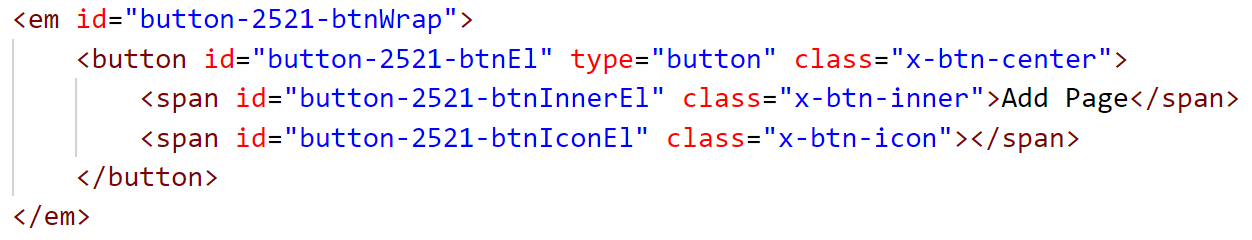
\includegraphics[width=15cm]{Chapter5/Pictures/picture52.png}
		\end{center}
		\caption{Đoạn mã HTML thể hiện Button Add Page của eXe}
		\label{refhinhchuong711}
	\end{figure}
\end{center}

Hình 5.2 ở trên thể hiện button Add Page của eXe, chúng ta có thể thấy ID của nó là button-2521-btnWrap, đây là 1 ID động và rất khó khăn để có thể xác định chính xác, vì mỗi lần chạy eXe, nó lại sinh ra 1 ID khác.\\

Để xử lý vấn đề này, chúng ta cần có những phương pháp phức tạp hơn. Trong luận văn này trình bày 2 phương pháp sau đây.

\begin{center}
	\begin{figure}[htp]
		\begin{center}
			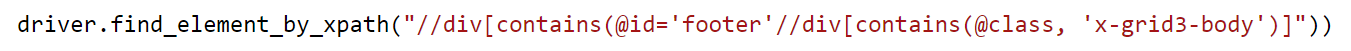
\includegraphics[width=15cm]{Chapter5/Pictures/picture53.png}
		\end{center}
		\caption{Đoạn mã Python thể hiện cách xác định một phần tử có 2 thuộc tính}
		\label{refhinhchuong65}
	\end{figure}
\end{center}

Phương pháp thứ nhất là xác định phần tử bằng nhiều thuộc tính cùng 1 lúc. Hình 5.3 ở trên thể hiện cách xác định 1 phần tử có thuộc tính thứ nhất là thẻ div có \textbf{id=’footer’}, thuộc tính thứ hai là thẻ div có class là \textbf{‘x-grid3-body’}. Phương pháp này đòi hỏi phải biết chính xác các thuộc tính mà phần tử đó có và quan trọng nó phải là duy nhất so với các phần tử còn lại.\\

\begin{center}
	\begin{figure}[htp]
		\begin{center}
			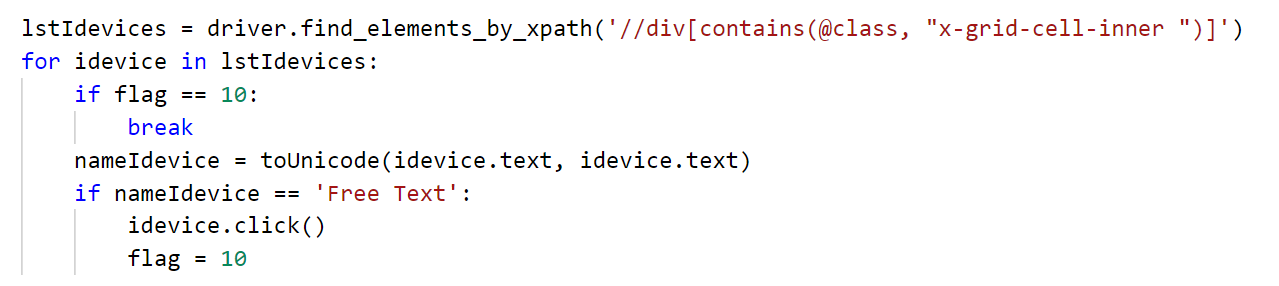
\includegraphics[width=15cm]{Chapter5/Pictures/picture54.png}
		\end{center}
		\caption{Đoạn mã Python thể hiện cách dùng thuộc tính text để xác định một phần tử}
		\label{refhinhchuong66}
	\end{figure}
\end{center}

Phương pháp thứ hai là dựa vào một thuộc tính riêng của một phần tử. Hình 5.4 ở trên thể hiện cách xác định 1 phần tử có thuộc tính \textbf{text} là \textbf{‘Free Text’}, vì có rất nhiều phần tử có chung thuộc tính là \textbf{class = ‘x-grid-cell-inner’}, do đó sẽ cho tất cả phần tử này vào cùng 1 danh sách (List), sau đó sẽ duyệt từng phần tử trong List này, nếu phần tử nào có thuộc tính là \textbf{text = ‘Free Text’} thì chúng ta sẽ chọn. Phương pháp này giúp chúng ta xác định mọi loại phần tử, tuy nhiên sẽ gây chậm nếu có quá nhiều phần tử có chung một thuộc tính. Do đó cần cân nhắc giữa hai phương pháp để xác định các phần tử hiệu quả nhất.

\newpage 

\subsection{Giải quyết về thiết kế số lượng mẫu kiểm tra}


Trong phần thách thức đã nêu ở trên, nếu một khóa học có n bài học thì sẽ có $n! * 9^n$ cách sắp xếp thứ tự các bài trong khóa học này. Con số này là quá lớn, cần có những phương pháp lập luận để giảm số lượng testcase xuống ít hơn.\\

Thông thường người soạn thảo thiết kế một khóa học có 5 bài học. Vì vậy lúc này số lượng tiền điều kiện xảy ra sẽ là $5!$. Tuy nhiên để đảm bảo về mặt chuyên môn, cần có những thiết kế khác để đảm bảo chất lượng của khóa học, không phải bài học nào cũng cần phải thay đổi vị trí với nhau. Thông thường "Bài 1" sẽ là bài để mở đầu khóa học, giới thiệu chung về khóa học nên vị trí của nó sẽ luôn là đầu tiên trong khóa học và "Bài 5" sẽ là bài tổng kết của khóa học, do đó vị trí của nó sẽ luôn nằm cuối cùng trong khóa học. Như vậy ta chỉ cần đảo vị trí của các bài học ở giữa là "Bài 2","Bài 3" và "Bài 4" với nhau.\\

Trong trường hợp kiến thức của các "Bài 2","Bài 3" và "Bài 4" có liên quan với nhau, cần phải tiếp thu theo một trình tự nhất định. Hình 5.5 ở dưới thể hiện một ví dụ trong trường hợp này.

\begin{center}
	\begin{figure}[htp]
		\begin{center}
			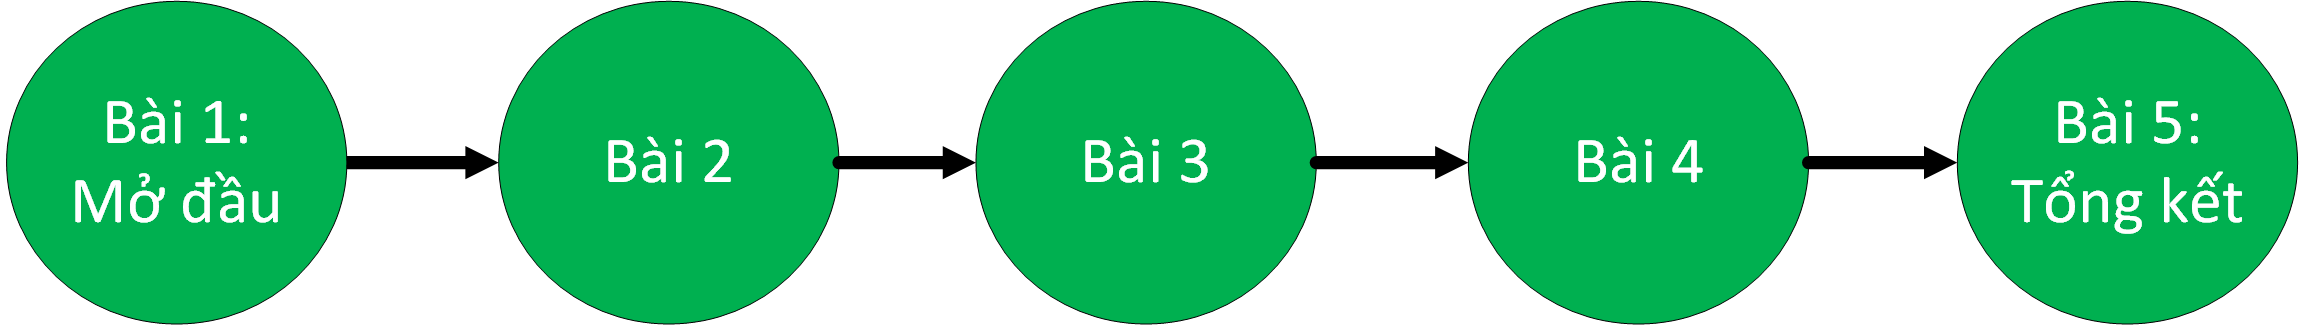
\includegraphics[width=16cm]{Chapter5/Pictures/picture55.png}
		\end{center}
		\caption{Nội dung các "Bài 2","Bài 3" và "Bài 4" liên quan với nhau}
		\label{refhinhchuong66}
	\end{figure}
\end{center}

Hình 5.5 thể hiện các trường hợp thiết lập tiền điều kiện cho các "Bài 2","Bài 3" và "Bài 4" có nội dung liên quan với nhau. Người học cần học 3 bài này theo một trình tự nhất định. Khi đó vị trí của bài học này sẽ thay đổi với nhau, ta sẽ hoán vị các vị trí của 3 bài học này. Như vậy ở đây ta sẽ có $3!=6$ trường hợp.\\

Trường hợp thứ hai là kiến thức của hai bài trong ba bài "Bài 2","Bài 3" và "Bài 4" độc lập với nhau. Lấy ví dụ nội dung của hai bài là "Bài 2" và "Bài 3" độc lập với nhau, khi đó sau khi học "Bài 1: Mở đầu", người học có thể lựa chọn học "Bài 2" hoặc "Bài 3" tiếp theo, vì nội dung của hai bài này độc lập với nhau, không liên quan với nhau. Như vậy ở đây ta sẽ có $3!=6$ trường hợp. Hình 5.6 ở dưới thể hiện các trường hợp có thể xảy ra.

\newpage

\begin{center}
	\begin{figure}[htp]
		\begin{center}
			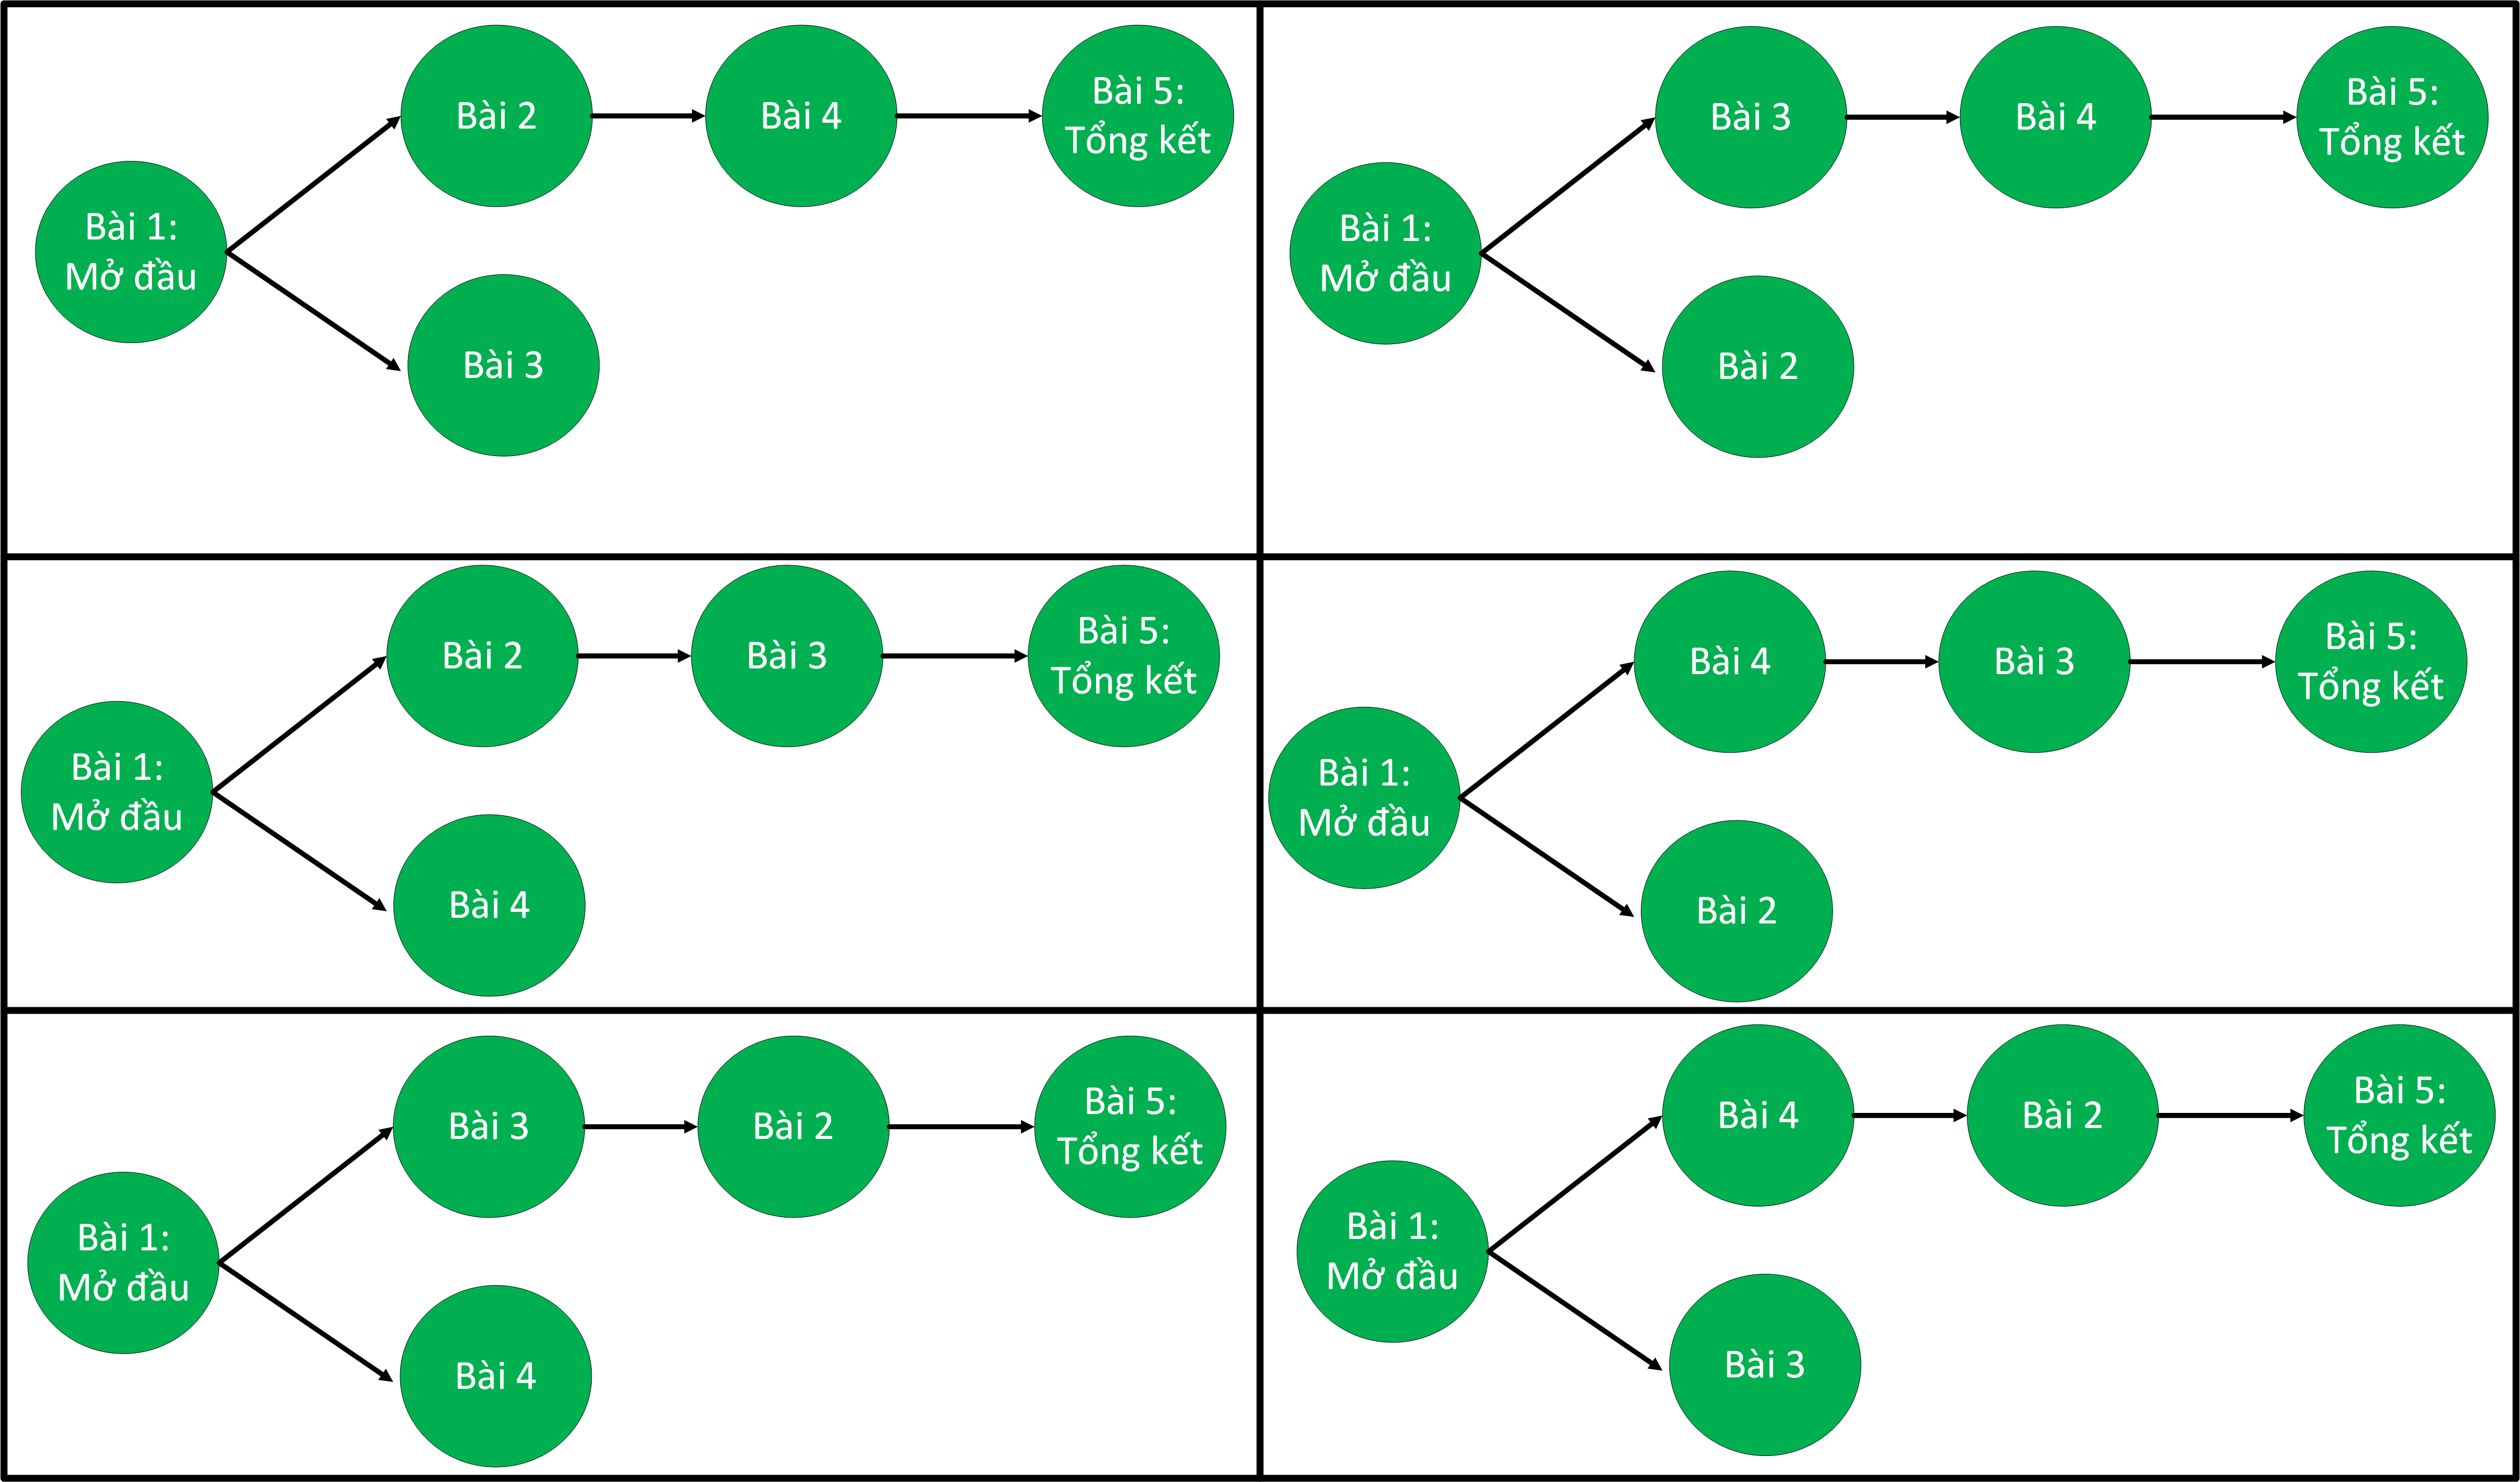
\includegraphics[width=16cm]{Chapter5/Pictures/picture56.png}
		\end{center}
		\caption{Nội dung hai bài trong ba bài độc lập với nhau}
		\label{refhinhchuong66}
	\end{figure}
\end{center}	



Trường hợp thứ ba là kiến thức của cả ba bài "Bài 2","Bài 3" và "Bài 4" độc lập với nhau. Khi đó sau khi học "Bài 1: Mở đầu", người học có thể lựa chọn học "Bài 2", "Bài 3" hoặc "Bài 4" tiếp theo vì nội dung của ba bài này độc lập với nhau, không liên quan với nhau. Như vậy ở đây ta sẽ có $3$ trường hợp. Hình 5.8 ở dưới thể hiện các trường hợp có thể xảy ra ở đây.

\begin{center}
	\begin{figure}[htp]
		\begin{center}
			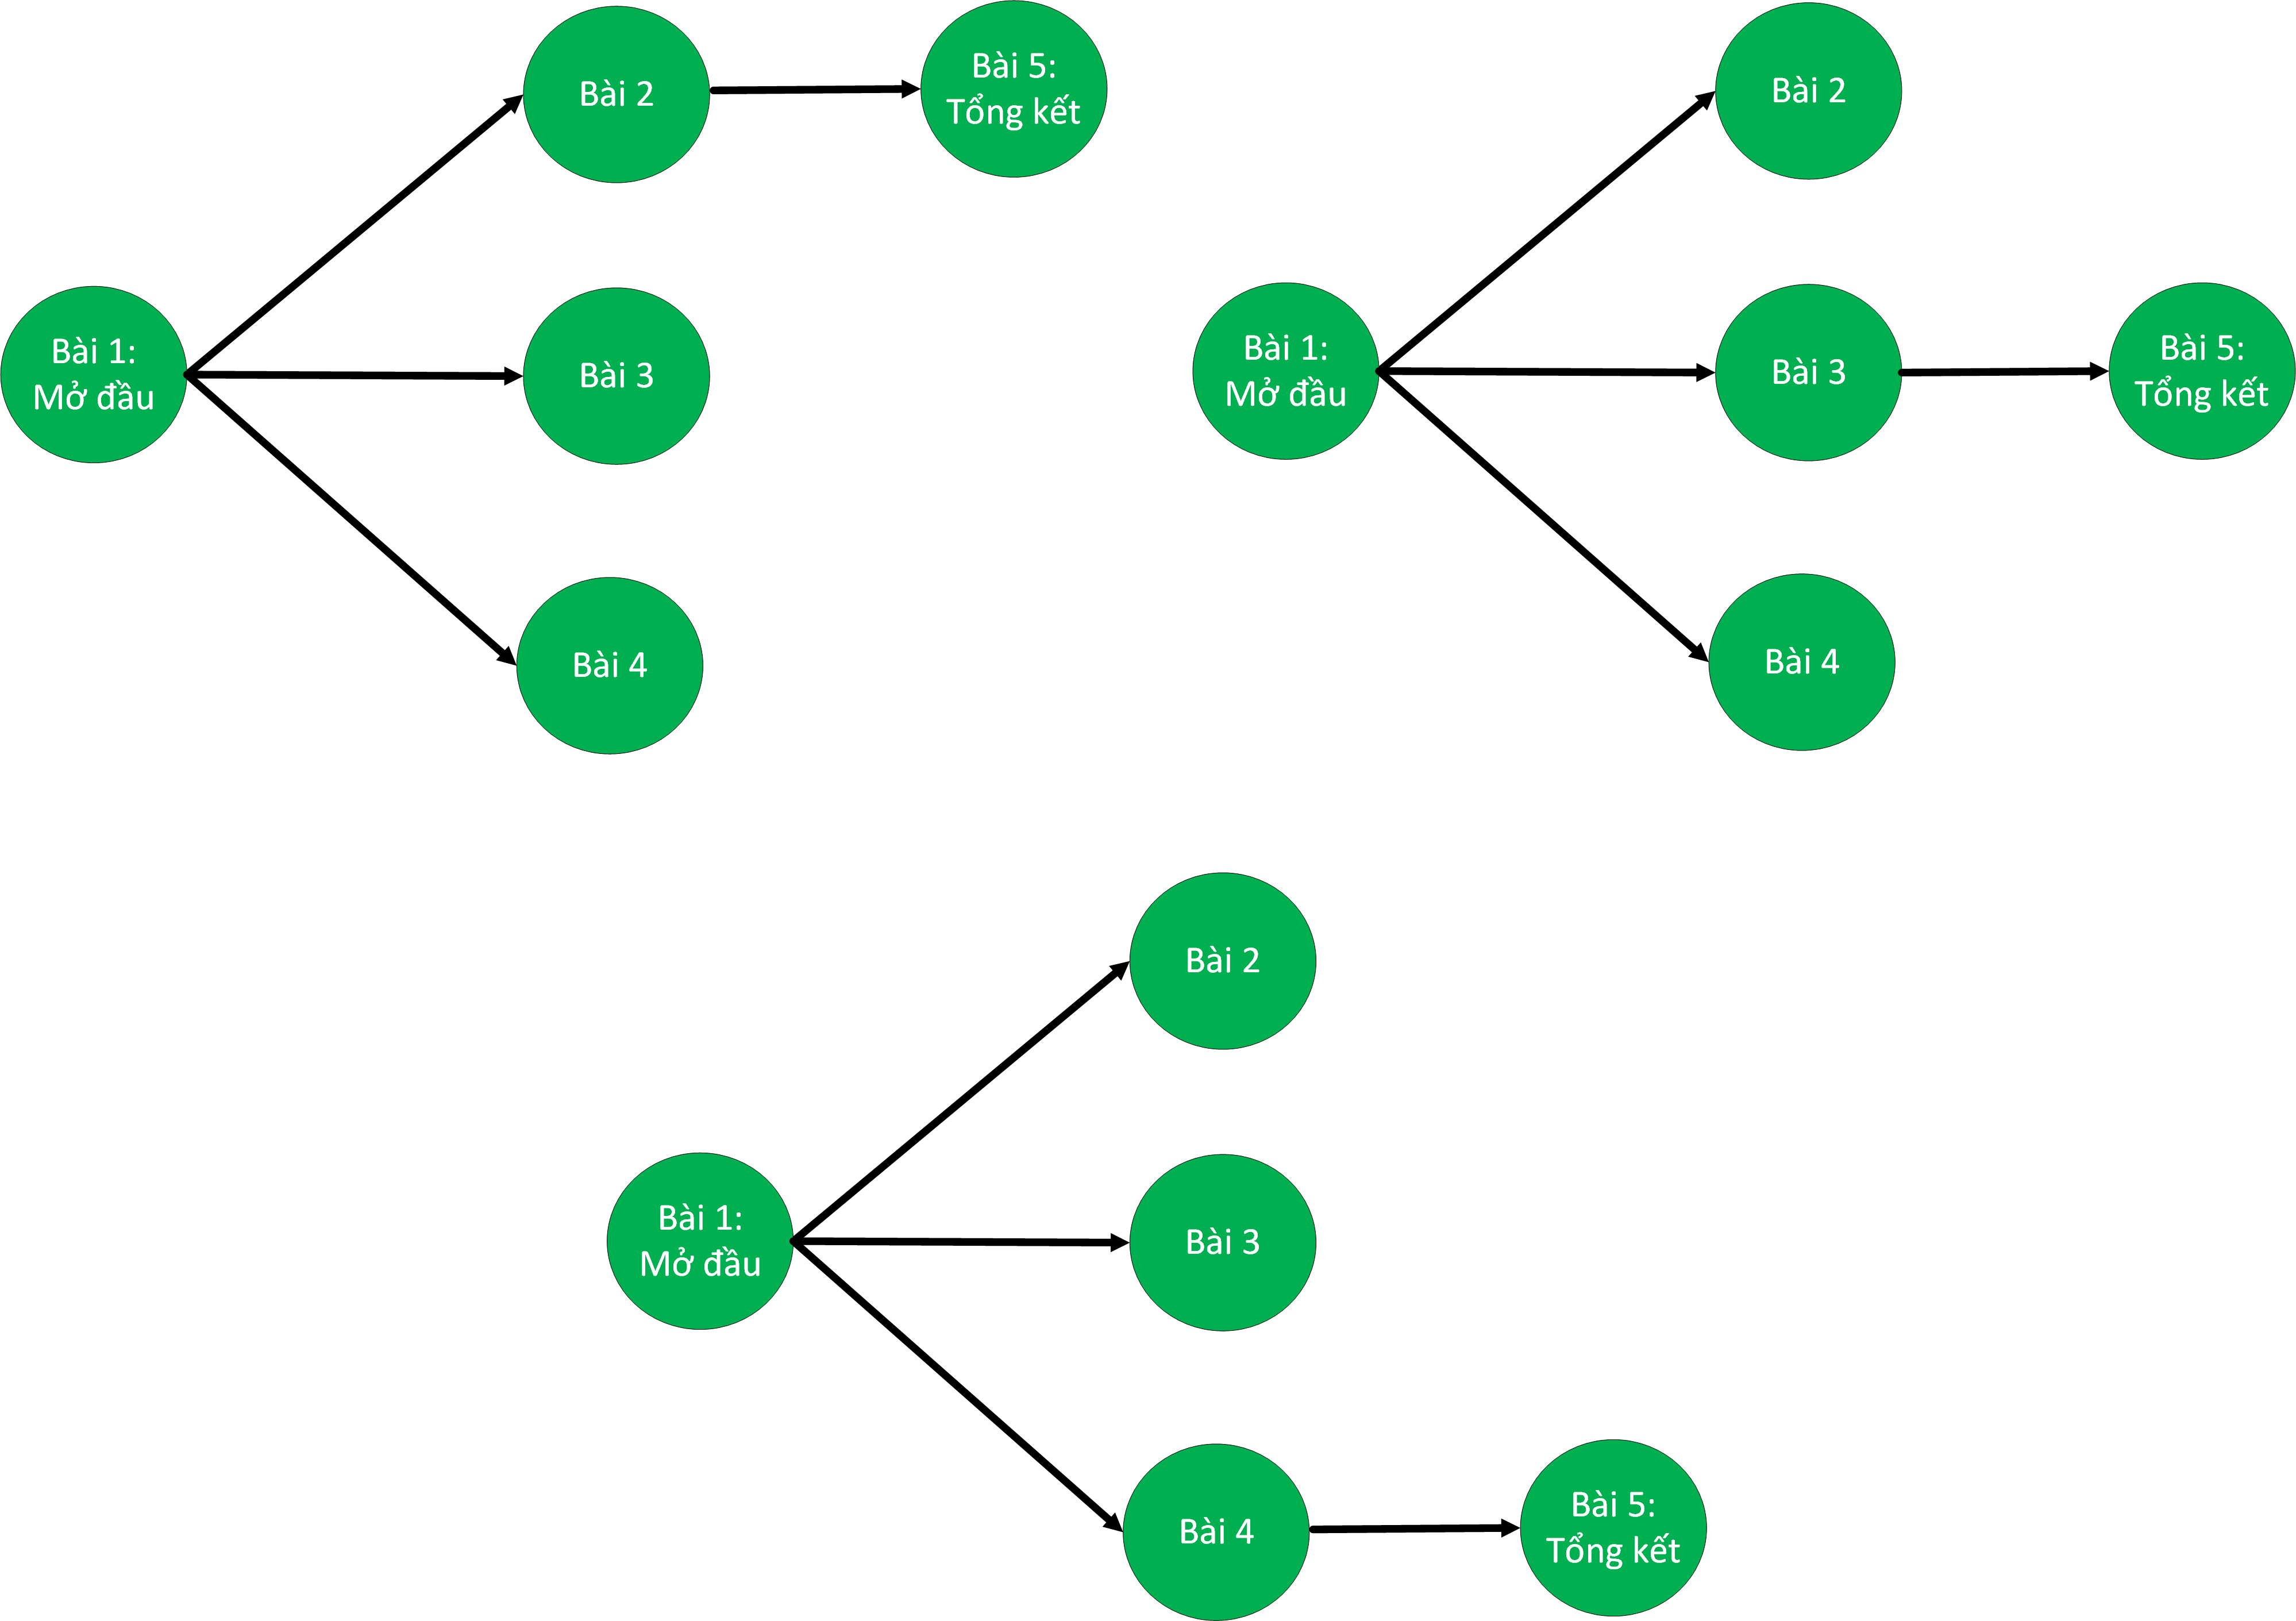
\includegraphics[width=10cm]{Chapter5/Pictures/picture57.png}
		\end{center}
		\caption{Nội dung cả ba bài độc lập với nhau}
		\label{refhinhchuong66}
	\end{figure}
\end{center}

\newpage

Như vậy trong trường hợp một khóa học có 5 bài học, ta sẽ có 15 trường hợp thiết lập tiền điều kiện cho khóa học này. Việc tiếp theo là thiết lập hậu điều kiện cho mỗi bài học trong khóa học.\\

Hậu điều kiện là điều kiện xác nhận người học đã hoàn thành bài học này, hậu điều kiện có thể là thời gian tối thiểu người học phải bỏ ra cho một bài học hoặc phải đạt một số bài kiểm tra nào đó do người biên soạn quy định. Đối với khóa học này, vì "Bài 1: Mở đầu" là bài giới thiệu tổng quan về khóa học, cho người học có một cái nhìn tổng quan về toàn bộ khóa học, vì vậy sẽ cần thiết lập thời gian ở bài này để người học dành nhiều thời gian tại đây, đảm bảo cho người học tìm hiểu về khóa học. Như vậy hậu điều kiện của "Bài 1: Mở đầu" sẽ là thời gian học tối thiểu (5 giây). Tiếp theo các "Bài 2","Bài 3" và "Bài 4" là những bài có kiến thức quan trọng trong khóa học, ở mỗi bài sẽ có 3 bài kiểm tra. Tuy nhiên vì số lượng câu hỏi cũng như độ khó của ba bài kiểm tra này do người soạn thảo đưa ra là như nhau, vì vậy hậu điều kiện cho các "Bài 2","Bài 3" và "Bài 4" này đều "Pass any quiz", có nghĩa là người học chỉ cần đạt 1 trong số 3 bài kiểm tra thì được xem là hoàn thành bài học. "Bài 5: Tổng kết" là bài ôn tập kiến thức tổng quan của cả khóa học, vì vậy ở đây sẽ có bài kiểm tra tổng hợp, không cần hậu điều kiện cho bài tổng hợp này.\\

Vậy hậu điều kiện của các bài học trong khóa học này đều là như nhau trong mọi trường hợp. "Bài 1: Mở đầu" có hậu điều kiện là thời gian tối thiểu phải bỏ ra (5 giây), "Bài 2","Bài 3" và "Bài 4" có hậu điều kiện là đạt một bài kiểm tra bất kỳ trong ba bài kiểm tra và cuối cùng là "Bài 5: Tổng kết" không có hậu điều kiện. Do đó chỉ có 1 trường hợp để thiết lập hậu điều kiện cho tất cả các bài trong khóa học này.\\

Như vậy sẽ có tổng cộng 15 testcase để kiểm thử cho phần mềm. Hình 5.8 thể hiện 15 testcase này.

\begin{center}
	\begin{figure}[htp]
		\begin{center}
			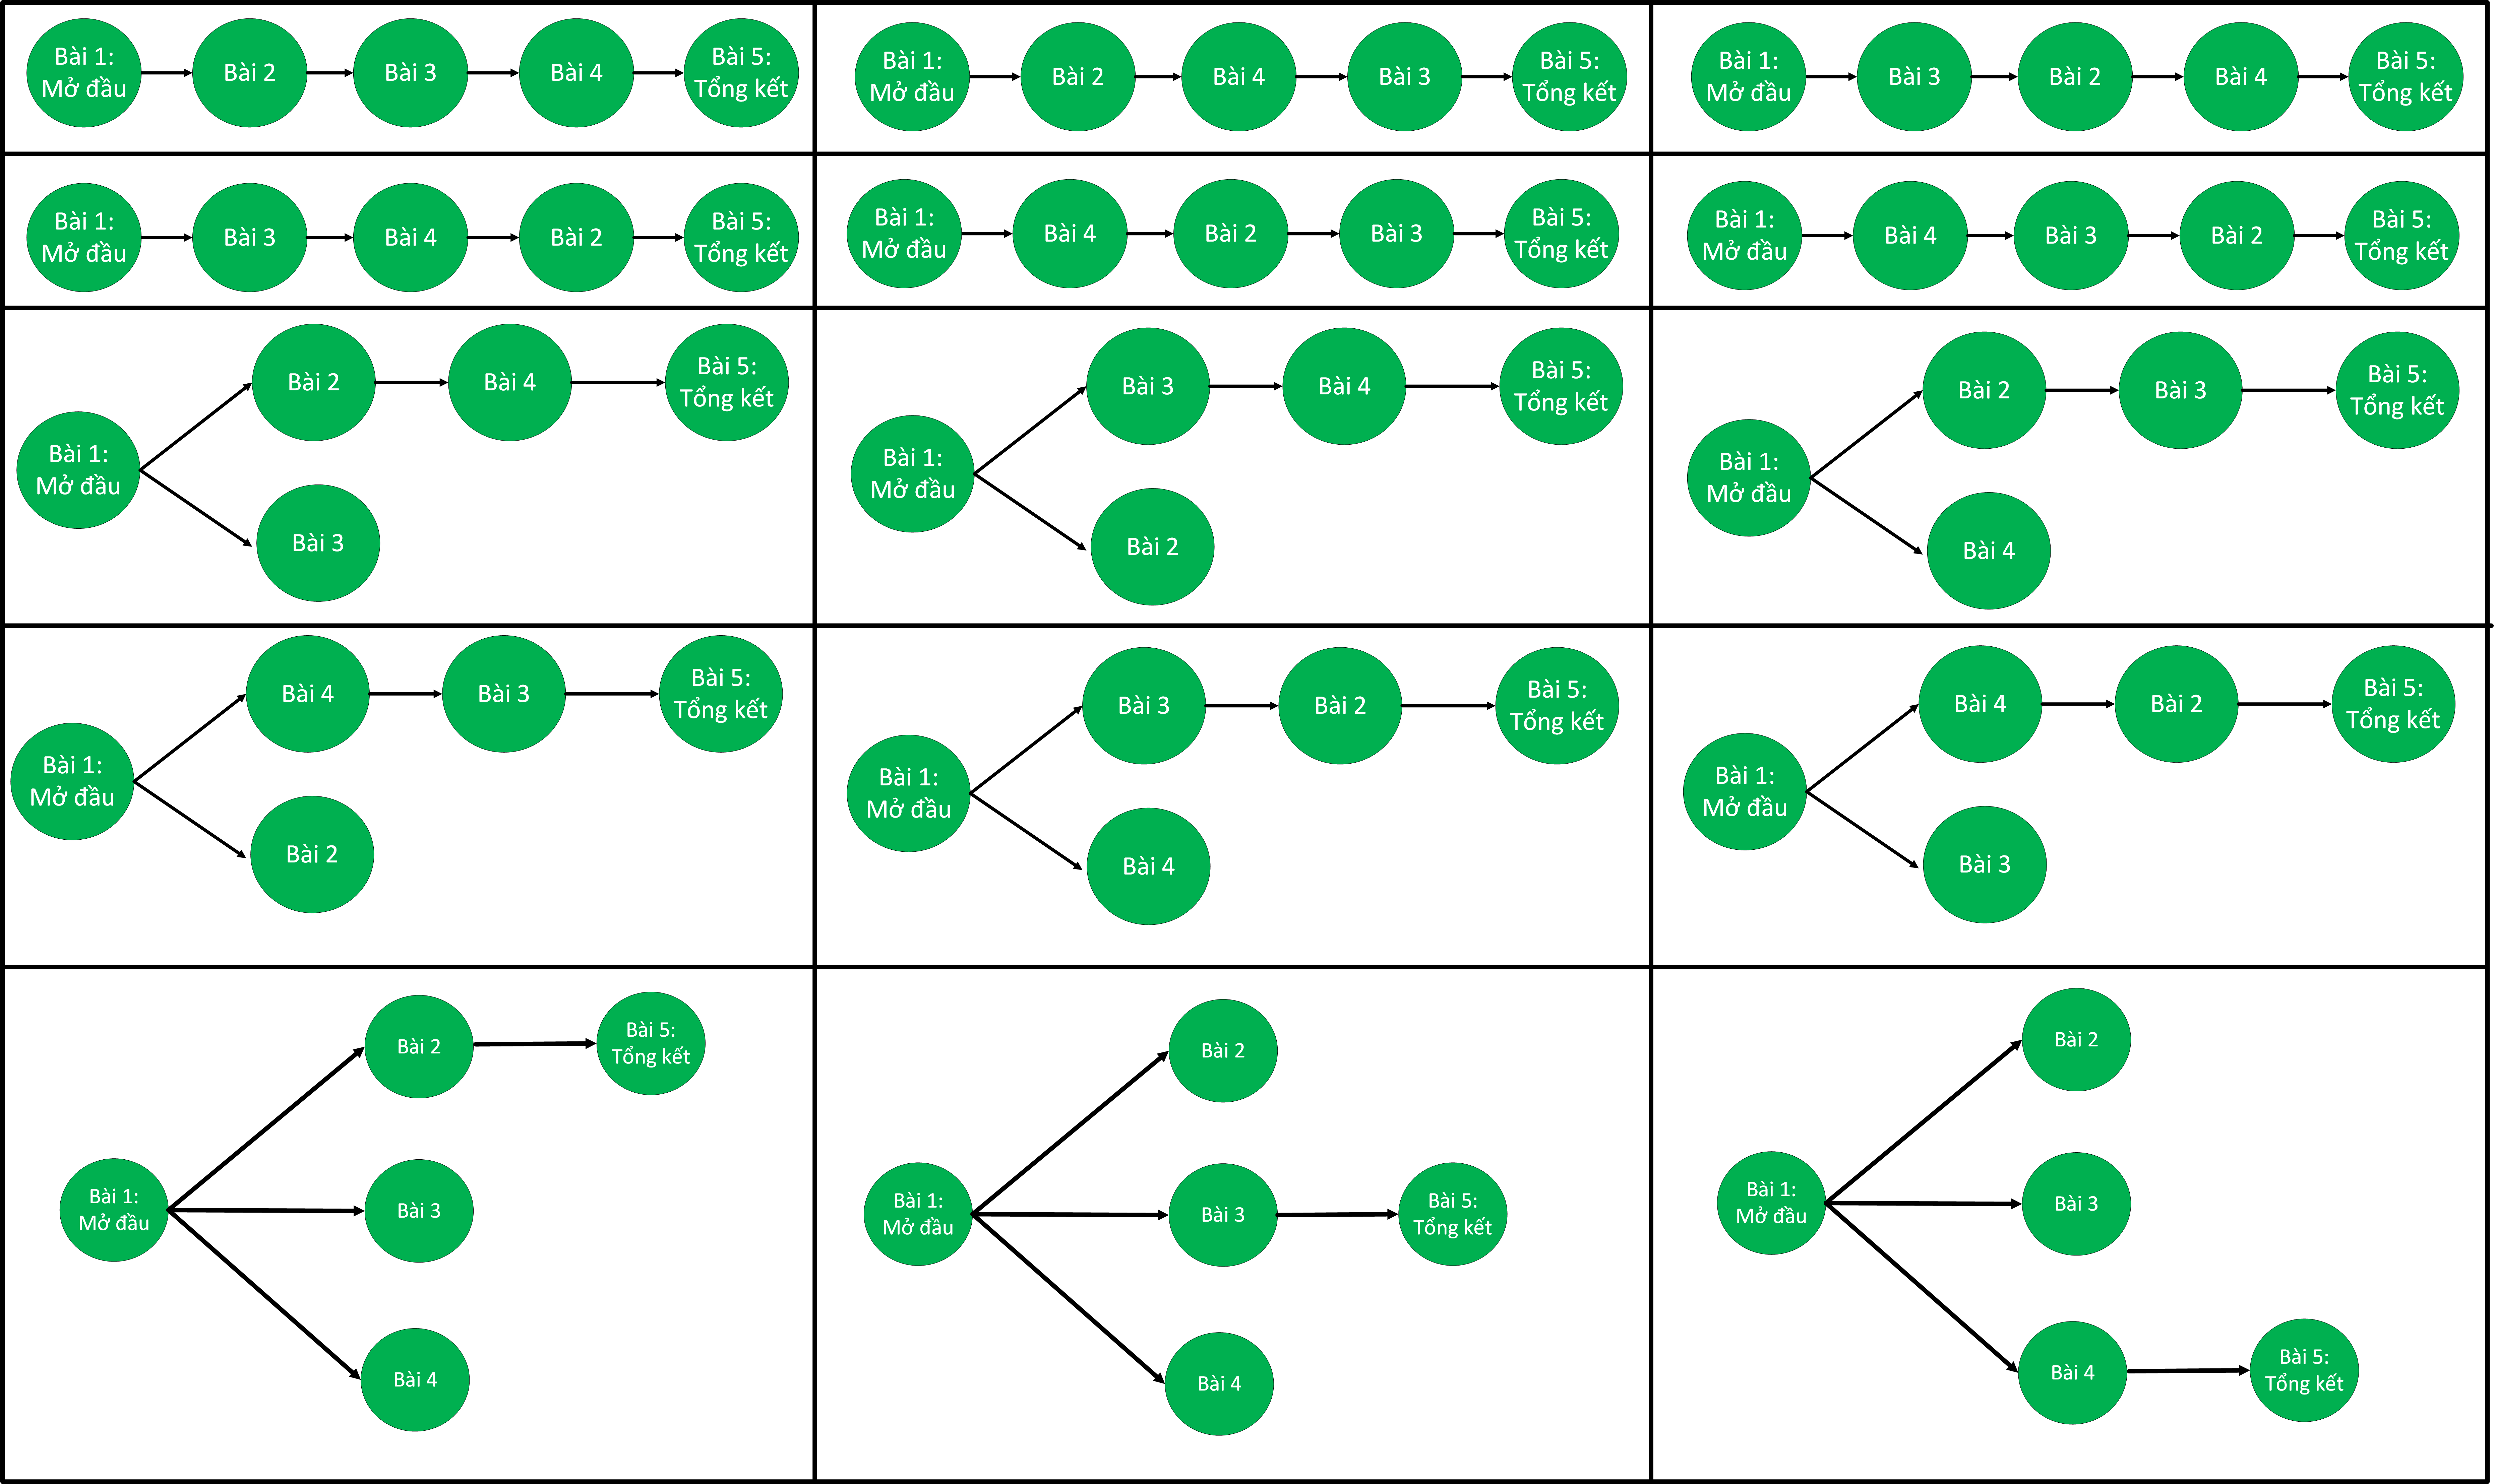
\includegraphics[width=16cm]{Chapter5/Pictures/picture58.png}
		\end{center}
		\caption{Tổng cộng các testcase}
		\label{refhinhchuong66}
	\end{figure}
\end{center}


\newpage

\section{Ví dụ mẫu kiểm tra}

\begin{comment}

\subsection{Chức năng điều khiển có điều kiện}

Như đã trình bày ở phần chiến lược kiểm thử, công việc kiểm thử bao gồm 2 giai đoạn. Giai đoạn thứ nhất là sử dụng eXe để soạn nội dung cho bài giảng, thiết lập các trang, sau đó đóng gói bài giảng theo chuẩn SCORM 2004. Giai đoạn thứ hai là upload bài học lên SCORM Cloud và tham gia bài học. Cả 2 giai đoạn đều được tự động hóa bằng Selenium WebDriver.

\subsubsection{Giai đoạn 1 - Tạo và đóng gói khóa học bằng eXe}

Mục đích của giai đoạn này là nhằm kiểm thử cho việc tạo mã SCORM, đảm bảo mã SCORM được sinh ra như ý muốn.\\

Giai đoạn này bao gồm 3 bước, được thể hiện như hình 6.7 ở dưới.

\begin{center}
\begin{figure}[htp]
\begin{center}
\includegraphics[width=15cm]{7xx11.png}
\end{center}
\caption{3 bước thực hiện của giai đoạn 1}
\label{refhinhchuong67}
\end{figure}
\end{center}

\vspace{1cm}

Hình 6.7 mô tả 3 bước thực hiện của giai đoạn 1. Bước thứ nhất là người biên soạn sẽ thực hiện việc thiết kế trang, soạn thảo nội dung cho khóa học bằng eXe. Tiếp theo bước thứ hai là người biên soạn sẽ thiết lập điều hướng cho các bài học, việc này giúp cho người học phải học các bài theo thứ tự đã quy định, nhằm đảm bảo tiếp thu được kiến thức theo một trình tự hợp lý do người soạn thảo đưa ra. Cuối cùng bước thứ ba là đóng gói khóa học theo chuẩn SCORM 2004 dưới dạng file zip, sau đó upload lên SCORM Cloud để người học có thể tham gia vào. Tất cả các bước đều được tự động hóa bằng Selenium WebDriver.\\

Sau đây sẽ trình bày ví dụ một mẫu kiểm tra.

\newpage

\textbf{Bước 1 - Thiết lập nội dung}\\

\begin{center}
\begin{figure}[htp]
\begin{center}
\includegraphics[width=10cm]{711.png}
\end{center}
\caption{Cấu trúc cây khóa học của mẫu kiểm tra trên eXe}
\label{refhinhchuong68}
\end{figure}
\end{center}

Hình 6.8 thể hiện cấu trúc cây khóa học của mẫu kiểm tra khi soạn thảo bằng eXe, mẫu này có tổng cộng 4 chương và 7 bài, bước tiếp theo là thiết lập điều hướng cho các bài.

\newpage

\textbf{Bước 2 - Thiết lập điều hướng}\\

\begin{center}
\begin{figure}[htp]
\begin{center}
\includegraphics[width=16cm]{7xx1.png}
\end{center}
\caption{Thiết lập trình tự các bài học}
\label{refhinhchuong7xx1}
\end{figure}
\end{center}

Hình 6.9 cho thấy thiết lập trình tự các bài học cho mẫu kiểm tra. Mẫu kiểm tra này được thiết lập thứ tự các bài học từ trên xuống dưới, thứ tự các bài học được đánh số từ 1 đến 10, người học cần học theo trình tự này và cần phải học đầy đủ các bài mới được xem là hoàn thành khóa học.\\

\newpage 

\textbf{Bước 3 - Đóng gói khóa học theo chuẩn SCORM 2004}

\begin{center}
\begin{figure}[htp]
\begin{center}
\includegraphics[width=15cm]{test2.png}
\end{center}
\caption{Đóng gói khóa học thành file zip}
\label{refhinhchuong7xx2}
\end{figure}
\end{center}

Bước cuối cùng của giai đoạn 1 là đóng gói khóa học theo chuẩn SCORM 2004 dưới dạng file zip. Hình 6.10 mô tả khóa học được đóng gói theo chuẩn SCORM thành file zip và được đặt tên là testconditionnavigate.zip.

\subsubsection{Giai đoạn 2 - Kiểm tra gói trên SCORM Cloud}

Mục đích của giai đoạn này là nhằm kiểm thử cho việc gói SCORM đã tạo, đảm bảo mã SCORM chạy đúng như thiết lập ban đầu.

Giai đoạn này bao gồm 2 bước, được thể hiện như hình 6.11 ở dưới.

\begin{center}
\begin{figure}[htp]
\begin{center}
\includegraphics[width=15cm]{test3.png}
\end{center}
\caption{2 bước thực hiện của giai đoạn 2}
\label{refhinhchuong611}
\end{figure}
\end{center}

Hình 6.11 mô tả 2 bước thực hiện của giai đoạn 2. Bước thứ nhất là upload gói bài học đã được đóng gói lên SCORM Cloud. Bước thứ hai là tham gia vào khóa học đã được upload trên SCORM Cloud. Hai bước đều được tự động hóa bằng Selenium WebDriver.\\

\newpage

\textbf{Bước 1 - Upload mẫu kiểm tra lên SCORM Cloud}\\

\begin{center}
\begin{figure}[htp]
\begin{center}
\includegraphics[width=16cm]{test4.png}
\end{center}
\caption{Khóa học được upload trên SCORM Cloud}
\label{refhinhchuong7xx}
\end{figure}
\end{center}


Hình 6.12 thể hiện cấu trúc của mẫu kiểm tra sau khi upload trên SCORM Cloud. Bước cuối cùng là cần hoàn thành khóa học đã upload.\\

\textbf{Bước 2 - Hoàn thành khóa học trên SCORM Cloud}\\

\begin{center}
\begin{figure}[htp]
\begin{center}
\includegraphics[width=16cm]{test5.png}
\end{center}
\caption{Hoàn thành khóa học trên SCORM}
\label{refhinhchuong7xx}
\end{figure}
\end{center}

Hình 6.13 thể hiện 2 trạng thái của khóa học, hình bên trái là trạng thái ban đầu của khóa học và hình bên phải là khóa học sau khi hoàn thành.
\newpage

\end{comment}


Sau đây là ví dụ về quá trình hiện thực kiểm tra một testcase trong bộ 15 testcase mà nhóm đã thiết kế. Hình 5.9 là mô tả của tổ chức khóa học mà nhóm lựa chọn để trình bày.

\begin{center}
	\begin{figure}[htp]
		\begin{center}
			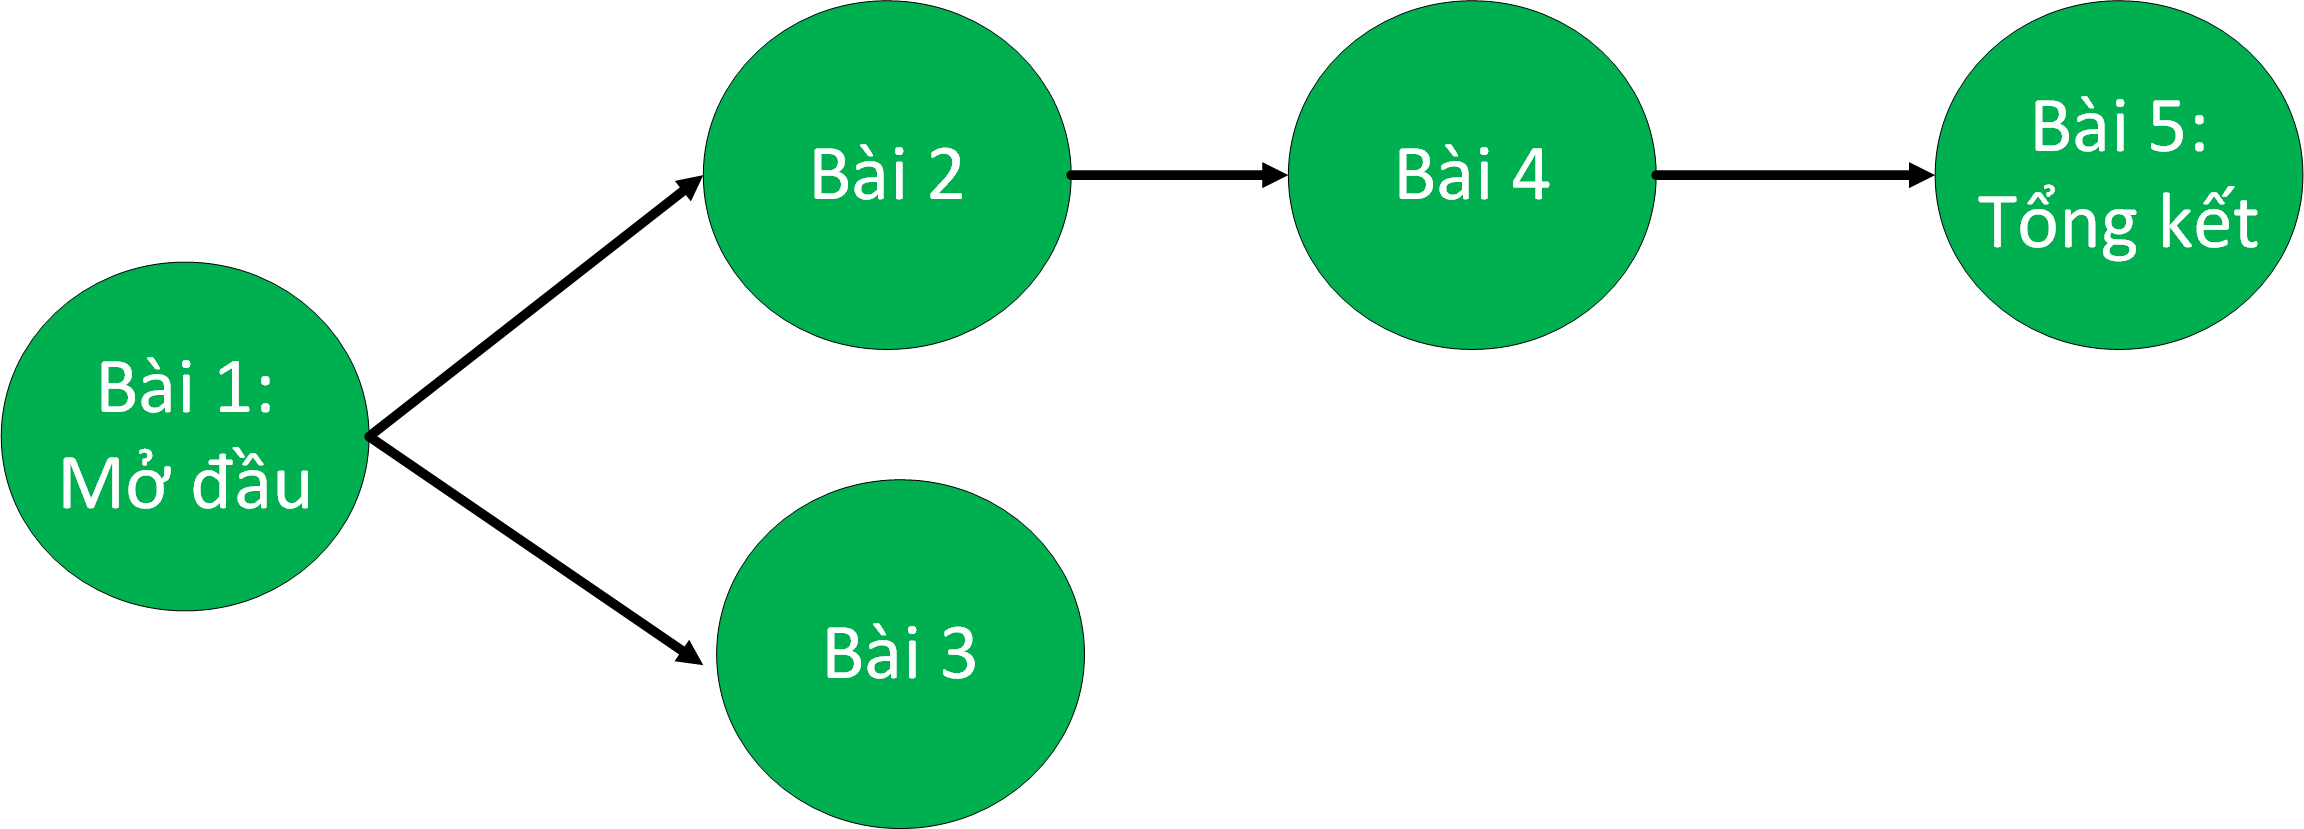
\includegraphics[width=15cm]{Chapter5/Pictures/picture59.png}
		\end{center}
		\caption{Tổ chức khóa học được sử dụng}
		\label{refhinhchuong66}
	\end{figure}
\end{center}

Tiếp theo sẽ thực hiện việc Upload tổ chức khóa học này lên SCORM Cloud.

\begin{center}
	\begin{figure}[htp]
		\begin{center}
			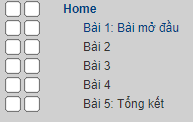
\includegraphics[width=10cm]{Chapter5/Pictures/picture510.png}
		\end{center}
		\caption{Khóa học hiển trị trên SCORM Cloud khi bắt đầu}
		\label{refhinhchuong66}
	\end{figure}
\end{center}

Hình 5.10 là gói SCORM sau khi được upload lên SCORM Cloud, theo mô hình trên thì chỉ có Bài 1: Bài mở đầu ở chế độ enable, còn các Bài 2, Bài 3, Bài 4 và Bài 5: Tổng kết sẽ ở chế độ disable do các tiền điều kiện ở các bài này chưa được thõa mãn. Như vậy SCORM Cloud đã thể hiện đúng trình tự mà người biên soạn thiết lập.

\newpage

\begin{center}
	\begin{figure}[htp]
		\begin{center}
			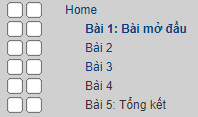
\includegraphics[width=10cm]{Chapter5/Pictures/picture511.png}
		\end{center}
		\caption{Khóa học được hiển trị trên SCORM Cloud khi học xong bài mở đầu}
		\label{refhinhchuong66}
	\end{figure}
\end{center}

Hình 5.11 là hiển thị trên SCORM Cloud sau khi người học xong Bài 1: Bài mở đầu. Các tiền điều kiện của Bài 2 và Bài 3 đã được thỏa mãn nên các bài này sẽ được chuẩn sang chế độ enable và người học có thể lựa chọn các bài này để học. Các tiền điều kiện của Bài 4 và Bài 5: Tổng kết vẫn chưa được thỏa mãn nên vẫn ở chế độ disable. Như vậy SCORM Cloud đã thể hiện đúng trình tự mà người biên soạn thiết lập.

\begin{center}
	\begin{figure}[htp]
		\begin{center}
			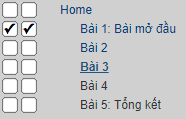
\includegraphics[width=10cm]{Chapter5/Pictures/picture512.png}
		\end{center}
		\caption{Khóa học được hiển trị trên SCORM Cloud khi học xong Bài 3}
		\label{refhinhchuong66}
	\end{figure}
\end{center}

Hình 5.12 là hiển thị trên SCORM Cloud sau khi người học học xong Bài 3. Lúc này Bài 4 và Bài 5 Tổng kết vẫn ở chế độ disable, theo mô hình tổ chức ở hình 5.9 thì các tiền điều kiện ở các bài này vẫn chưa được thỏa mãn. Như vậy SCORM Cloud đã thể hiện đúng trình tự mà người biên soạn thiết lập.

\newpage

\begin{center}
	\begin{figure}[htp]
		\begin{center}
			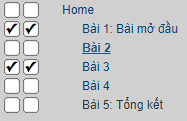
\includegraphics[width=10cm]{Chapter5/Pictures/picture513.png}
		\end{center}
		\caption{Khóa học được hiển trị trên SCORM Cloud khi học xong Bài 2}
		\label{refhinhchuong66}
	\end{figure}
\end{center}


Hình 5.13 là hiển thị trên SCORM Cloud sau khi người học học xong Bài 2. Lúc này Bài 4 sẽ được chuyển sang chế độ enable do các tiền điều kiện đã được thỏa mãn. Bài 5: Tổng kết vẫn ở chế độ disable do tiền điều kiện bài này vẫn chưa thỏa mãn.

\begin{center}
	\begin{figure}[htp]
		\begin{center}
			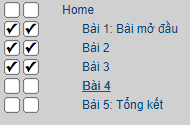
\includegraphics[width=10cm]{Chapter5/Pictures/picture514.png}
		\end{center}
		\caption{Khóa học được hiển trị trên SCORM Cloud khi học xong Bài 4}
		\label{refhinhchuong66}
	\end{figure}
\end{center}


Hình 5.14 là hiển thị trên SCORM Cloud sau khi người học học xong Bài 4. Lúc này tiền điều kiện của Bài 5: Tổng kết sẽ được thỏa mãn và Bài 5 sẽ được chuyển sang chế độ enable. Như vậy SCORM Cloud đã thể hiện đúng trình tự mà người biên soạn thiết lập theo tổ chức bài học đưa ra ở hình 5.9.

\newpage


\subsubsection{Nhận xét và kết luận}

Quá trình kiểm thử cho việc tạo một bài giảng điện tử bằng eXe và sử dụng bài giảng trên SCORM Cloud mang lại kết quả tốt. Việc thiết kế các trang, thiết lập điều khiển có điền kiện cho các bài học,... Sau đó upload bài giảng lên SCORM Cloud, tham gia vào bài giảng và hoàn thành bài giảng đúng như thiết lập của người soạn thảo, việc này cho thấy mã SCORM đã được sinh ra chính xác và chạy đúng như các thiết lập ban đầu. Tuy nhiên mặt hạn chế là kịch bản kiểm thử khá dài, đòi hỏi cần phải có kỹ năng lập trình để có thể xây dựng một kịch bản kiểm thử chính xác và hiệu quả.\\

Trong quá trình thực hiện vẫn còn có một số sai sót. Nhưng với việc tìm hiểu về của các trường hợp sai đó, thì nguyên nhân là từ các lý do khách quan đã được lường trước như mạng chậm, không kết nối được vào mạng. Tuy nhiên các trường hợp sai sót này có thể được xử lý tốt bằng cách thiết lập thời giai chờ đợi hợp lý trong kịch bản kiểm thử để có được kết quả tốt nhất, ít sai sót nhất.\\

Các mẫu kiểm thử còn lại được thực hiện như quy trình của mẫu kiểm thử trên.






































